\footnotesize
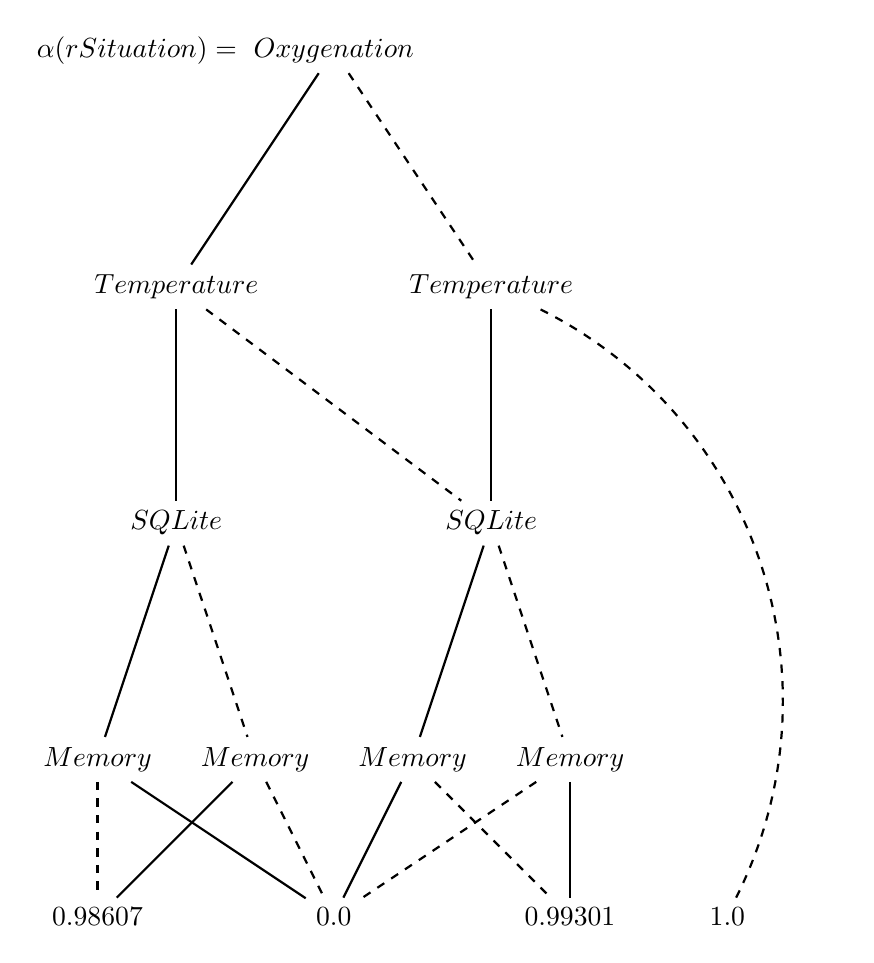
\begin{tikzpicture}[thick]
%\draw[help lines, step=1cm] (0,0) grid +(14,12);
\node[rectangle,draw=none](alpha) at (1.5,12) {$\alpha(rSituation)=$};
\node(o1) at (4,12) {$Oxygenation$};
\node(t1) at (2,9) {$Temperature$};
\node(t2) at (6,9) {$Temperature$};
\node(sq1) at (2,6) {$SQLite$};
\node(sq2) at (6,6) {$SQLite$};
\node(m1) at (1,3) {$Memory$};
\node(m2) at (3,3) {$Memory$};
\node(m3) at (5,3) {$Memory$};
\node(m4) at (7,3) {$Memory$};
\node[rectangle, draw=none](tr1) at (1,1) {$0.98607$};
\node[rectangle, draw=none](tr2) at (4,1) {$0.0$};
\node[rectangle, draw=none](tr3) at (7,1) {$0.99301$};
\node[rectangle, draw=none](tr4) at (9,1) {$1.0$};

\draw(o1)--(t1);
\draw[dashed](o1)--(t2);
\draw(t1)--(sq1);
\draw[dashed](t1)--(sq2);
\draw(t2)--(sq2);
\draw[dashed](t2) to [bend left=45](tr4);
\draw(sq1)--(m1);
\draw[dashed](sq1)--(m2);
\draw(sq2)--(m3);
\draw[dashed](sq2)--(m4);
\draw[dashed](m1)--(tr1);
\draw(m1)--(tr2);
\draw(m2)--(tr1);
\draw[dashed](m2)--(tr2);
\draw(m3)--(tr2);
\draw[dashed](m3)--(tr3);
\draw[dashed](m4)--(tr2);
\draw(m4)--(tr3);
\end{tikzpicture}
\normalsize
